\section{Experiments}\label{foi.exp}
In this section, I describe some simple experiments (methods and results) to
highlight differences in the various equations and approaches
to modelling HIV transmission in sexual partnerships.
%===================================================================================================
\subsection{Within- \vs Between-Partnership Heterogeneity}\label{foi.exp.xph}
For computing an average per-partnership probability of transmission ($B$),
\sref{foi.prior.xph} clarified the interpretations of
\eqref{eq:B.wph} \vs \eqref{eq:B.bph} as modelling
within-partnership heterogeneity (WPH) \vs between-partnership heterogeneity (BPH), respectively.
As shown in \sref{app.foi.proof} (proof), $B_{\wph} \ge B_{\bph}$.
Here I explore under what conditions the ratio $B_{\wph}~/~B_{\bph}$ is maximized
--- \ie when does choosing the correct approach matter most.
For simplicity, I considered a single illustrative factor $f$
affecting $\alpha_f \in [0,1]$ proportion of sex acts ($1-\alpha_f$ are unaffected),
with relative probability of transmission $R_f \in [0.01,~10]$.
I~then computed $B_{\wph}$ and $B_{\bph}$ for $A \in [1,1000]$ total sex acts,
using a base per-act probability of transmission $\beta = 0.34$\%
as a representative value for HIV \cite{Boily2009}.
\par
\begin{figure}
  \centering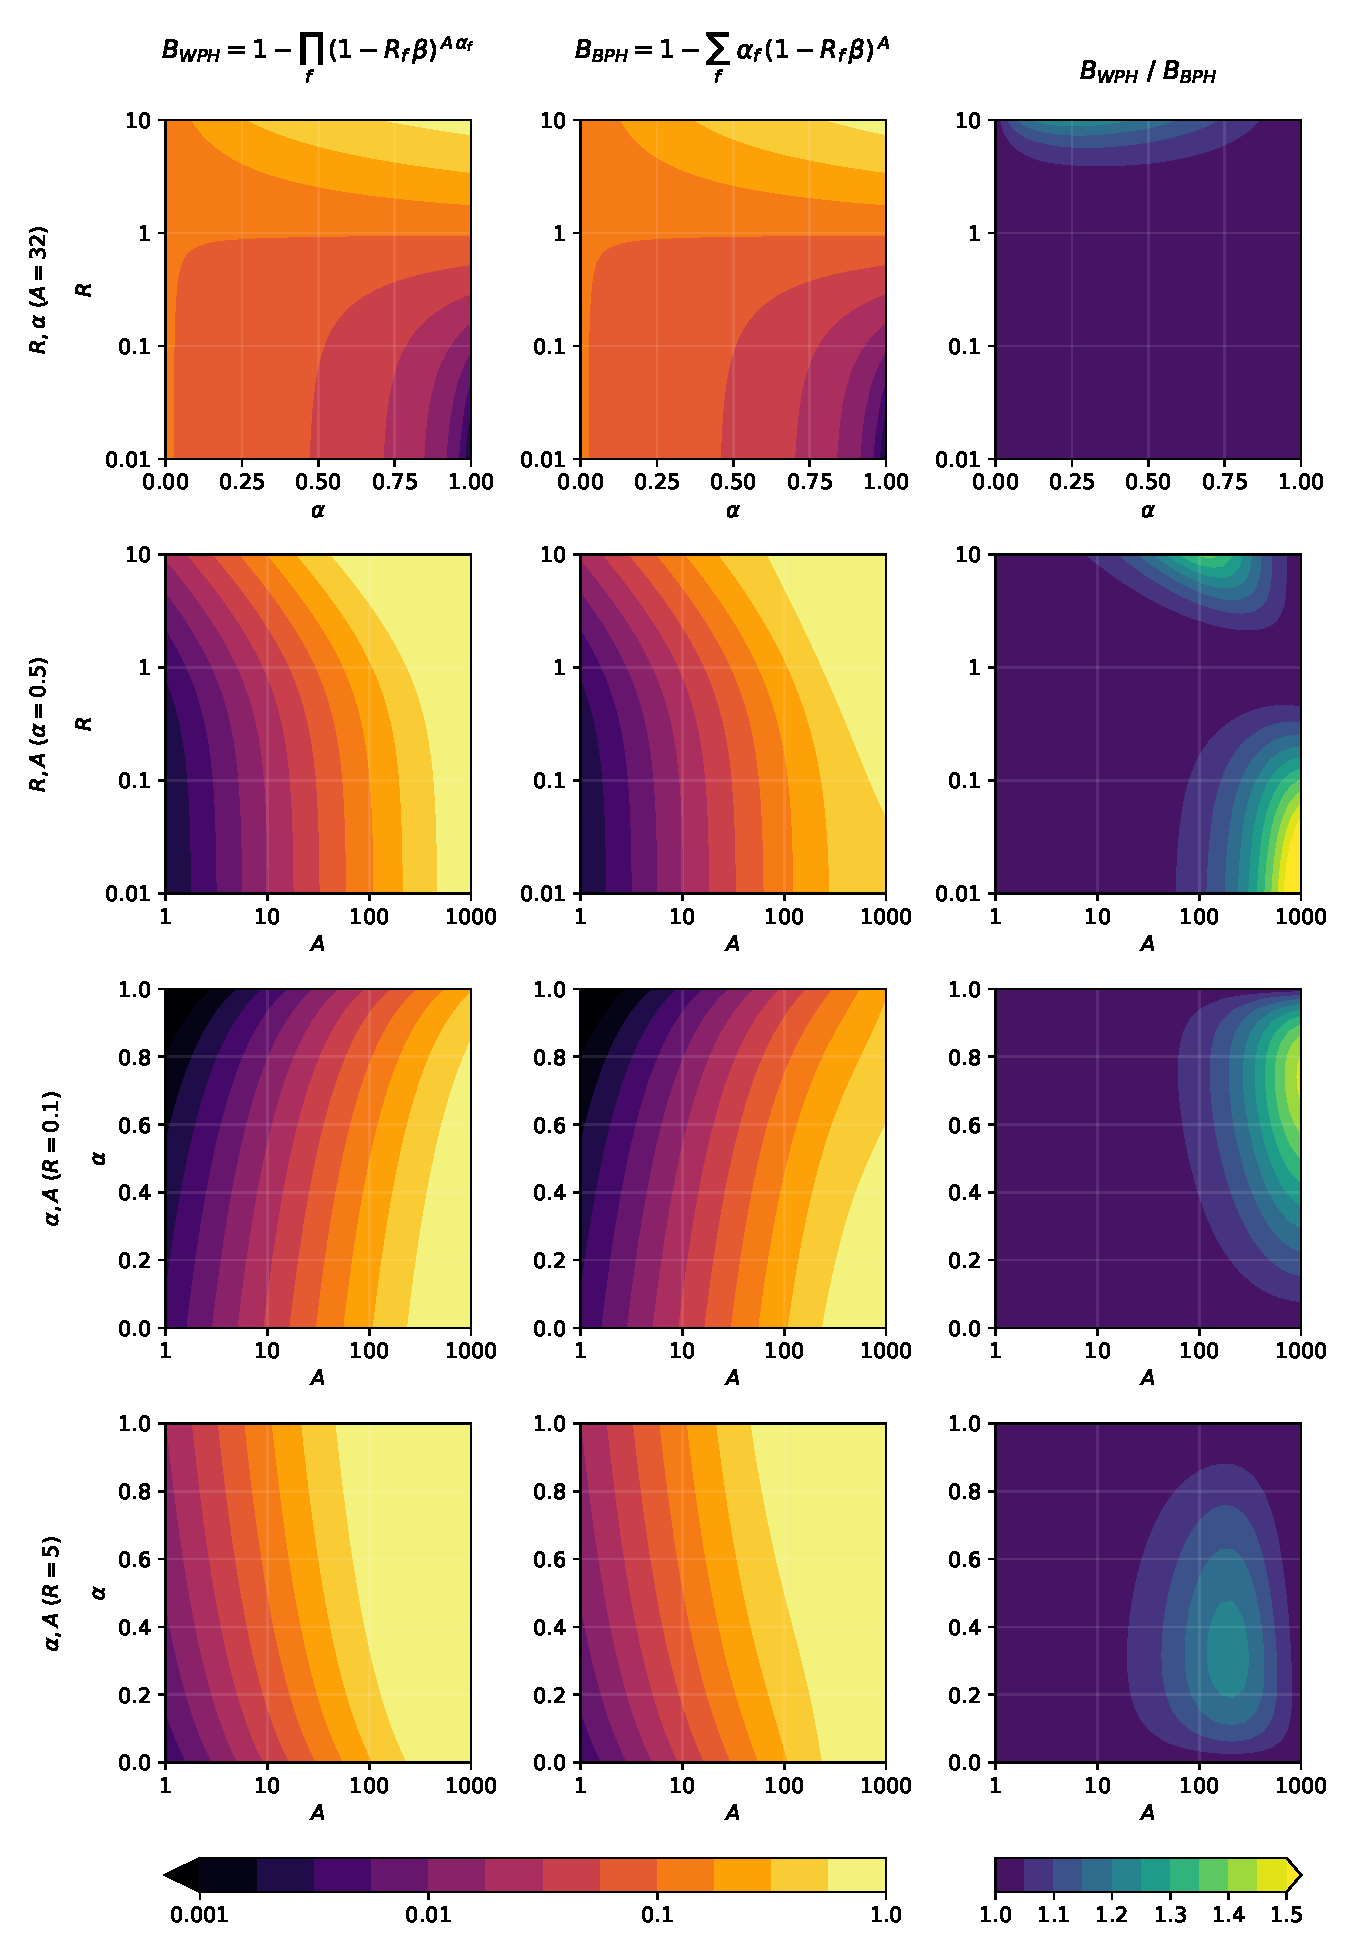
\includegraphics[scale=.6]{B.xph.surf.pdf}
  \caption{Average per-partnership probability of transmission $B$
    given heterogeneity in the per-act probability of transmission $\beta$
    within \vs between partnerships}
  \label{fig:B.xph.surf}
  \floatfoot{
    $B$: probability of transmission per partnership (log scale colourmap);
    $\beta = 0.34\%$: probability of transmission per sex act (fixed) \cite{Boily2009};
    $A$: total sex acts per partnership (log scale);
    $\alpha_f$: proportion of sex acts affected by factor $f$ (linear scale);
    $R_f$: relative $\beta$ given factor $f$ (log scale);
    WPH: within-partnership heterogeneity;
    BPH: between-partnership heterogeneity.}
\end{figure}
\begin{figure}
  \centering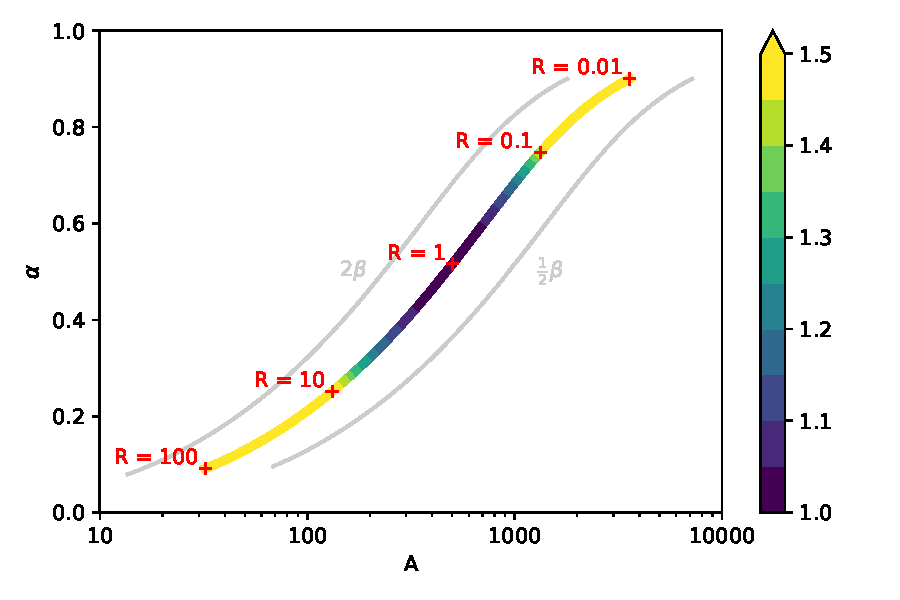
\includegraphics[scale=.6]{B.xph.max.pdf}
  \caption{Parameter values $(\alpha,A)$ which maximize the difference between
    the average per-partnership probability of transmission
    given within- \vs between-partnership heterogeneity}
  \label{fig:B.xph.max}
  \floatfoot{
    $B_{\wph}~/~B_{\bph}$: line colour;
    $\beta = 0.34\%$: probability of transmission per sex act (fixed) \cite{Boily2009};
    $A$: total sex acts per partnership (log scale);
    $\alpha_f$: proportion of sex acts affected by factor $f$ (linear scale);
    $R_f$: relative $\beta$ given factor $f$ (log scale);
    gray lines denote equivalent contours for $2\beta$ and $\frac12\beta$.}
\end{figure}
Figure~\ref{fig:B.xph.surf} illustrates four 2-dimensional cross sections of $B(R,\alpha,A)$
under WPH \vs BPH, and the ratio $B_{\wph} / B_{\bph}$;
the cross sections were at: $A = 32$, $\alpha = 0.5$, $R = 0.1$, and $R = 5$.
Based on these results, the difference between approaches can be summarized as:
\begin{itemize}
  \item negligible for $A < 10$, and small for $A < 100$
  \item increasing as $R$ gets farther from 1 ($R \rightarrow 0$ or $R \rightarrow \infty$)
  \item maximized by specific values of $(\alpha,A)$ for a given $R$, including
    $\alpha > \frac12$ for $R < 1$, and $\alpha < \frac12$ for $R > 1$
\end{itemize}
The specific values of $(\alpha,A)$ which maximize
the difference between approaches for a given $R$ and $\beta$
create a continuous curve (Figure~\ref{fig:B.xph.max}), which slowly tends towards
$\alpha \rightarrow 1, A \rightarrow \infty$ as $R \rightarrow 0$, and
$\alpha \rightarrow 0, A \rightarrow 0$ as $R \rightarrow \infty$.
The curve is sigmoidal for log-transformed $A$,
and shifts left with increasing $\beta$.
I did not derive an analytical expression, but it should be possible to do so.
In the context of HIV, the difference between approaches would be
larger for protective factors (\eg condoms)
affecting most of a large number of sex acts ($\alpha > 1000$);
and likewise larger for risk-increasing factors (\eg anal sex)
affecting a minority of a moderate number of sex acts ($\alpha \approx 100$).
%===================================================================================================
\subsection{Partnership Durations}\label{foi.exp.dur}
As described in \sref{foi.prior.part}, multiple prior models have
implicitly assumed a maximum partnership duration $\delta \le 1$ year.
As such, the adjustment for PTC \eqref{eq:B} would have less effect.
This reduced effect can be quantified via
the effective probability of transmission per sex act $\beta'$
--- \ie tangent slopes in Figure~\ref{fig:binom.dur} --- defined as:
\begin{equation}\label{eq:beta.eff}
  \beta' = \frac{B}{A} = \frac{1 - {(1 - \beta)}^{A}}{A}
\end{equation}
Figure~\ref{fig:dur.surf} illustrates the 1-year $\beta'_1$ \vs true-duration $\beta'_\delta$, for
different partnership durations $\delta \in [1, 30]$ and sex frequencies $F \in [1,~180]$ per year.
% Evidently $\beta'_1$ does not depend on $\delta$.
Assuming $\delta \le 1$ can considerably increase the modelled rate of transmission
for partnerships with $F \ge 52$ (\ie weekly) and a true duration $\delta \ge 5$ years,
including up to \emph{8-fold} difference with $F \approx 100$ and $\delta \approx 30$.
Thus, prior models using $\delta \le 1$ may have
substantially overestimated the relative contribution of
longer partnerships with frequent sex --- including main/spousal partnerships ---
to overall transmission.
\begin{figure}
  \centering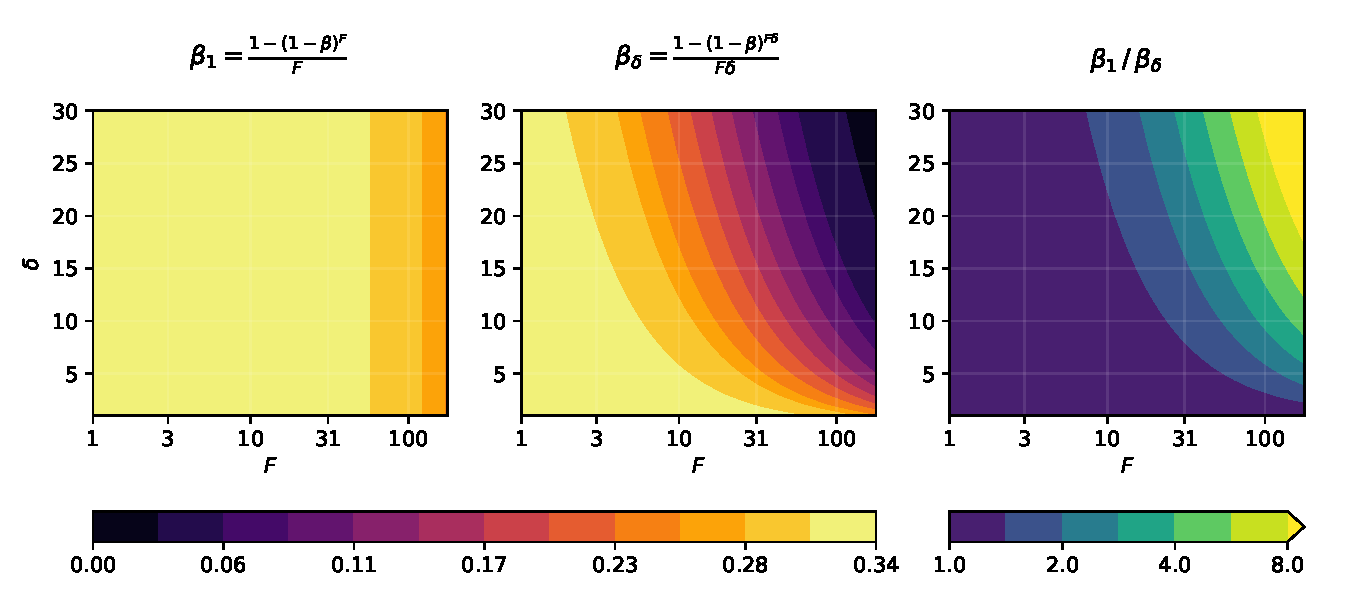
\includegraphics[scale=.6]{dur.surf.pdf}
  \caption{Effective probability of transmission per sex act
    over 1 year \vs total partnership duration}
  \label{fig:dur.surf}
  \floatfoot{
    $\beta = 0.34\%$: probability of transmission per sex act (fixed) \cite{Boily2009};
    $F$: frequency of sex per partnership (per year, log scale);
    $\delta$: partnership duration (years, linear scale);
    $\beta_1, \beta_\delta$: effective probability of transmission per sex act,
      for 1 year \vs total partnership duration, respectively.}
\end{figure}
\clearpage % TEMP
%===================================================================================================
\subsection{Comparing Approaches in a Complete Model}\label{foi.exp.model}
Next, I sought to explore how different approaches to
modelling HIV transmission via sexual partnerships --- \ie the force of infection ---
influence key outputs from a complete model.
For this analysis, I focused on two aspects of prior approaches:
whether or not partnership durations are effectively capped at 1 year (\sref{foi.prior.dur}), and
whether incidence is aggregated across partnerships as a rate \vs proportion (\sref{foi.prior.part}).
Thus, I considered 3 prior approaches,
plus the \emph{Effective Partnerships Adjustment} approach from \sref{foi.prop}
(Table~\ref{tab:foi.models}).
I integrated each approach within the model from Chapter~\ref{model}.
\begin{table}[h]
  \centering
  \caption{Compared approaches to modelling HIV transmission via sexual partnerships}
  \label{tab:foi.models}
  \begin{tabular}{clcl}
  \toprule
  ID & Name & Key Eqs. & Key Parameters \\
  \midrule
  \epa & Effective Partnerships Reduction & (\ref{eq:M.SI})--(\ref{eq:foi.jh})  & $K,F,\delta$ \\
  \ird & Instantaneous Rate-Duration      & (\ref{eq:B.bph}),~(\ref{eq:foi.ir}) & $A,Q$        \\
  \iry & Instantaneous Rate-1-Year        & (\ref{eq:B.bph}),~(\ref{eq:foi.ir}) & $A_1,Q_1$    \\
  \ipy & Instantaneous Proportion-1-Year  & (\ref{eq:B.bph}),~(\ref{eq:foi.ip}) & $A_1,Q_1$    \\
  \bottomrule
\end{tabular}
\floatfoot{
  $K$: number of concurrent partners;
  $F$: frequency of sex per partnership;
  $\delta$: partnership duration;
  $A = F\delta$: total sex acts per partnership;
  $Q = K/\delta$: partnership formation rate;
  $A_1 = F \delta_1$, $Q_1 = K/\delta_1$, where $\delta_1 = \min{(\delta,1)}$.}
\end{table}
\par
I then explored selected model outputs under each of the 4 approaches,
with the aim of characterizing:
\begin{enumerate}
  \item \label{obj:foi.dyn}
  fundamental differences in transmission dynamics under each approach
  \item \label{obj:foi.tpaf}
  differences in the model-estimated prevention priorities under each approach
\end{enumerate}
For aim~\ref{obj:foi.dyn}, I compared HIV incidence (overall and group-specific)
using \emph{equal} model parameters across approaches.
For aim~\ref{obj:foi.tpaf}, I compared
the transmission population attributable fraction (TPAF, details in \sref{foi.exp.model.tpaf})
of several transmission pathways,
using \emph{approach-specific} model parameters (recalibrated).
A transmission pathway could reflect a given partnership type,
or infections acquired among and/or transmitted from a given risk group, etc.
Since applied models are usually calibrated to a given context,
aim~\ref{obj:foi.tpaf} thus provides a realistic comparison of
how prevention priorities could differ when informed by models using each approach.
%---------------------------------------------------------------------------------------------------
\paragraph{Equal \vs Approach-Specific Parameters}
The \emph{Effective Partnerships Adjustment} (\epa) approach uses the
numbers of concurrent partnerships $K$,
frequency of sex per partnership $F$,
and partnership duration $\delta$,
while the prior approaches use the
total numbers of sex acts per-partnership $A$,
and partnership formation rate $Q$.
For \emph{equal} model parameters,
I used model fits (parameter sets) from \epa (see \sref{model.res.par}),
and converted $A = F \delta$ and $Q = K/\delta$ for all 3 prior approaches (\ird,~\iry,~\ipy),
with the additional adjustment $\delta_1 = \min{(\delta,1)}$ for the 1-year approaches (\iry,~\ipy).
For \emph{approach-specific} parameters, I repeated the methods in \sref{model.cal},
yielding 1000 unique model fits (parameter sets) for each prior approach.
Model calibration figures for HIV prevalence and incidence are given in \sref{app.foi.cal}.
%---------------------------------------------------------------------------------------------------
\subsubsection{Transmission Dynamics using Equal Parameters}\label{foi.exp.model.dyn}
Figure~\ref{fig:foi.ep.incidence} illustrates HIV incidence under each approach among
FSW, clients, and everybody else (``lower risk'').
Specifically, Figure~\ref{fig:foi.ep.incidence.raw} illustrates incidence per person-year
(\epa repeated for comparison)
and Figure~\ref{fig:foi.ep.incidence.rel} illustrates relative differences \vs the \epa approach.%
\footnote{Relative differences were ``paired'' according to each parameter set $k$,
  and computed as $(\textsc{ixx}_k - \epa_k) / \epa_k$.}
I made the following observations --- and \emph{hypothesized} explanations, drawing on
the complete network of modelled transmission under \epa (Figure~\ref{fig:wiw.base.alluvial}):
\begin{itemize}
  \item Incidence among lower risk was generally much higher under 1-year approaches (\iry,~\ipy)
    --- underestimation of PTC under these approaches
    disproportionately increases transmission via main/spousal partnerships,
    allowing more transmission to/from lower risk individuals,
    including a positive feedback loop via increasing HIV prevalence
    given like-width-like mixing (see \sref{model.par.mix.odds}).
  \item Incidence differences between the 1-year approaches (\iry,~\ipy) \vs \epa grew over time
    --- \epa explicitly models the accumulation of seroconcordant partnerships
    wherein sex acts are PTC, or ``partnership-level herd effects'' \cite{Knight2022smdm};
    thus, by underestimating PTC throughout the epidemic,
    the 1-year approaches are initially less biased \vs \epa, but later overestimate incidence.
  \item Incidence among all risk groups was lower under the full-duration approach (\ird)
    --- complete and instantaneous accounting of PTC under this approach
    effectively delays transmission in all partnership types,
    and contributes to a lower HIV prevalence feedback loop.
  \item Incidence among FSW and clients was lower under the ``incidence proportion'' approach (\ipy)
    --- incidence proportion \eqref{eq:foi.ip} treats all transmission risks as competing,
    and notably forces incidence $\lambda^\ip \le 1$,
    disproportionately reducing incidence among those at highest risk.
  \item Incidence among FSW and clients under \iry approximately matched \epa\ 
    --- competing biases due to underestimation of some PTC (delays transmission),
    but not all PTC (overestimates transmission)
    coincidentally yielded incidence roughly matching \epa.
\end{itemize}
Overall, \ird resulted in the most \emph{consistent} bias \vs \epa across groups and over time.
\begin{figure}
  \subcapoverlap
  \foreach \var in {raw,rel}{
  \begin{subfigure}{\linewidth}
    \centering
    \includegraphics[width=.975\linewidth]{foi.ep.incidence.\var.pdf}
    \caption{\raggedright}
    \label{fig:foi.ep.incidence.\var}
  \end{subfigure}}
  \caption{HIV incidence among selected risk groups,
    estimated under different prior force of infection approaches (colours)
    \vs the \emph{Effective Partnerships Adjustment} approach using equal model parameters}
  \label{fig:foi.ep.incidence}
  \floatfoot{\fffoi;
    \sfref{fig:foi.ep.incidence.raw} absolute incidence;
    \sfref{fig:foi.ep.incidence.rel} relative differences: $(\textsc{ixx}_k - \epa_k) / \epa_k$;
    \ffpopz; \ffribbon.}
\end{figure}
\par
Figure~\ref{fig:foi.wiw.part} further illustrates the proportions of modelled yearly HIV infections
transmitted via different partnership types under each approach
using equal parameters (top) and approach-specific parameters for comparison (bottom).
As hypothesized above, for equal parameters, the 1-year approaches (\iry,~\ipy) featured
the greatest proportions of transmission via main/spousal partnerships, and the least via sex work.
By contrast, the full-duration approach (\ird) featured
the smallest proportions transmitted via main/spousal partnerships, and the most via sex work.
The distribution under the proposed approach (\epa) was in between these two extremes.
Interestingly, there were minimal differences in Figure~\ref{fig:foi.wiw.part} between
1-year incidence rate (\iry) \vs incidence proportion (\ipy) approaches.
\begin{figure}
  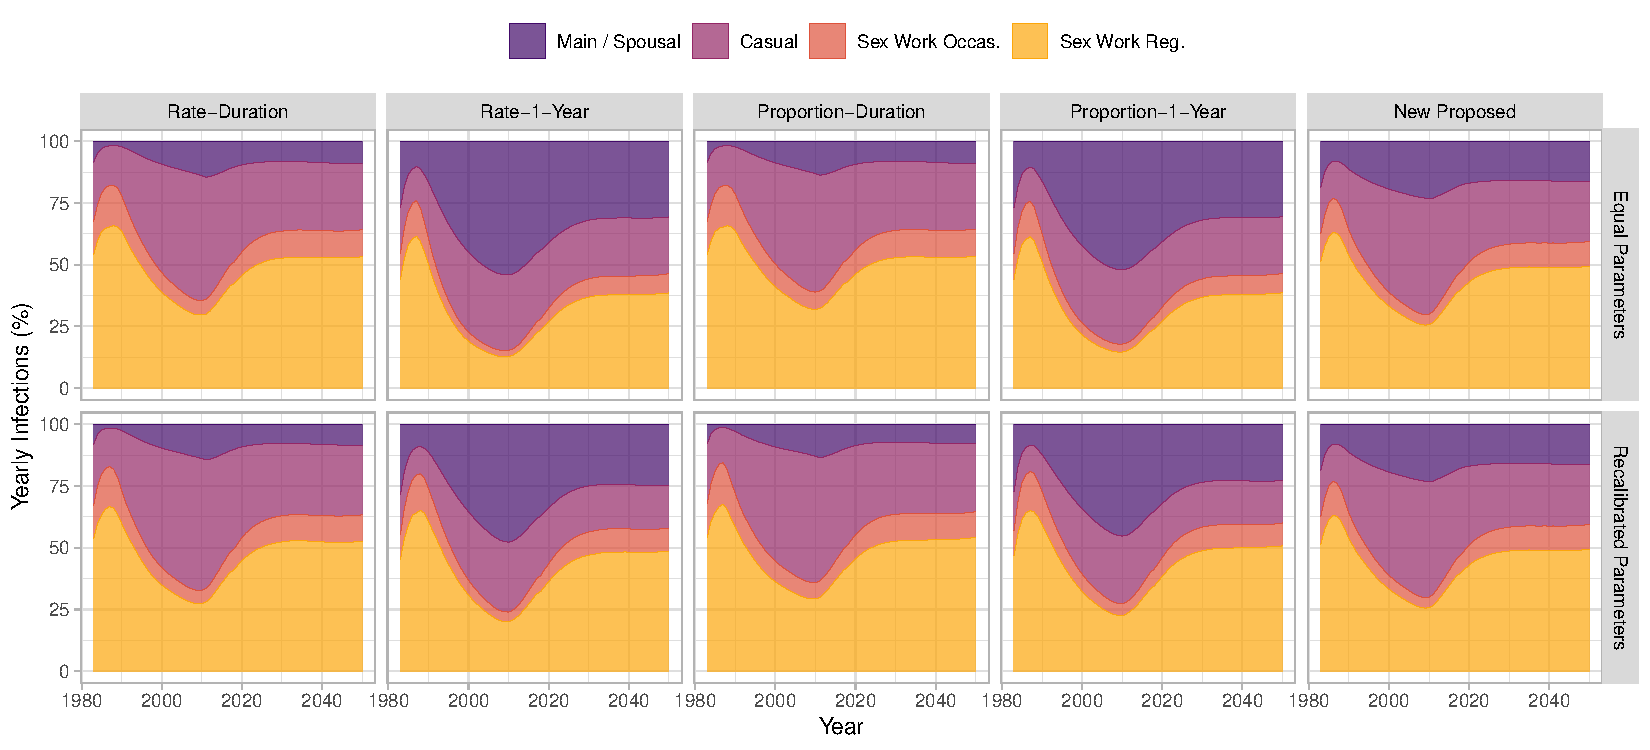
\includegraphics[width=\linewidth]{foi.wiw.part.pdf}
  \caption{Proportions of modelled yearly HIV infections
    transmitted via different partnership types in Eswatini
    estimated under different force of infection approaches (horizontal facets)
    with equal \vs recalibrated parameters (vertical facets)}
  \label{fig:foi.wiw.part}
  \floatfoot{\fffoi; \ffwiw.}
\end{figure}
%---------------------------------------------------------------------------------------------------
\subsubsection{Prevention Priorities using Approach-Specific Parameters}\label{foi.exp.model.tpaf}
Many models applied to assess HIV prevention priorities
explicitly model specific intervention scenarios, often with a cost dimension
\cite{Anderson2014,Kerr2015,Maheu-Giroux2019}.
However, these context-specific intervention and cost details
require additional analyses and/or assumptions,
and only explore a subset of the modelled transmission pathways.
By contrast, the TPAF reflects an ``intervention agnostic'' measure of
how any given transmission pathway contributes to transmission overall.
% TODO: calibration figures
%---------------------------------------------------------------------------------------------------
\paragraph{Transmission Population Attributable Fractions (TPAFs)}
Classic PAFs aim to quantify
the relative contribution of a specific factor to a given outcome at the population level,
by comparing the number of outcomes with \vs without the factor \cite{Rockhill2011,Poole2015}.
However, classic PAFs are not well-suited for infectious diseases,
especially over longer time horizons, because
they fail to capture the nonlinear dynamics of indirect transmission \cite{Mishra2020}.
In some cases, preventing one transmission event could avert numerous downstream infections;
in other cases, preventing one transmission event might only
delay infection a short time for an individual at high risk.
The TPAF for infectious diseases was developed as a better measure of the contribution of
different transmission pathways to overall transmission \cite{Deering2008,Mishra2014,Mishra2016}.
\par
The TPAF among population $j$ of transmission pathway $k$ is defined as
the relative difference in cumulative infections $\Omega$ among $j$ since a given time $t_0$
with vs without transmission via $k$:
\begin{equation}\label{eq:tpaf}
  \textup{TPAF}_{jk}(t) = \frac{\Omega_{j}(t) - \Omega_{jk} (t)}{\Omega_{j}(t)}
  ,\qquad
  \Omega_{jk}(t) = \int_{t_0}^{t} \Lambda_{j,M_k=0}(\tau)\,d\tau
  ,\qquad
  t = t_0 + \Delta_t
\end{equation}
Thus, TPAFs reflect hypothetical interventions with perfect prevention,
ignoring practical implementation challenges associated with any real intervention.
Like classic PAFs, TPAFs can sum to more than 100\% \cite{Rowe2004,Mishra2021}.
\par
I computed TPAFs for the following transmission pathways:
main/spousal, casual, and sex work (occasional and regular combined) partnership types; and
transmission from FSW, clients, and everybody else (``lower risk'').
I computed these TPAFs under each of the 5 force of infection approaches,
over $\Delta_t = {}$1, 3, and 10-year time horizons,
starting in $t_0 = {}$1990, 2000, and 2010 (270 total TPAFs).
I implemented scenarios without transmission via pathway $k$
using a boolean ``mask'' applied to the mixing matrix $M_{pii'}$,
\emph{after} resolving the values per \sref{model.par.mix},
such that mixing patterns were not affected.
%---------------------------------------------------------------------------------------------------
\paragraph{TPAFs of Partnership Types}
Figure~\ref{fig:foi.tpaf.part} illustrates the TPAFs for partnership types.
TPAFs generally increased over longer time horizons $\Delta_t$,
increased with calendar year $t_0$ for non-sex work partnerships, and
decreased with $t_0$ for sex work (\nb vertical scales).
Such trends are consistent with prior work showing that
TPAFs of key populations are typically large at first
and decrease as epidemics become more widespread
\cite{Johnson2011,Mishra2012sr,Boily2015}.
\foreach \var/\lab in {%
  part/transmission via different partnership types,%
  popf/transmission from different risk groups}{
\begin{figure}
  \includegraphics[width=\linewidth]{foi.tpaf.\var.pdf}
  \caption{TPAF of \lab\ (horizontal facets),
    starting from different $t_0$ (vertical facets),
    estimated under different force of infection approaches (colours)}
  \label{fig:foi.tpaf.\var}
  \floatfoot{\fffoi; \fftpaf; \ffbox.}
\end{figure}}
\par
TPAF differences across force of infection approaches were largest for main/spousal partnerships,
with 1-year approaches (\iry,~\ipy) significantly larger than the full-duration approach (\ird).
Main/spousal TPAFs under \epa were similar to \iry~and~\ipy from 1990 over short time horizons,
beyond which TPAFs under \epa were more similar to \ird;
similar to incidence differences in \sref{foi.exp.model.dyn},
these findings reflect reduced transmission via longer partnerships over time
due to the accumulation of seroconcordant partnerships, which are only captured under \epa.
Relative differences in casual partnership TPAFs across approaches
were exactly opposite (but less pronounced) \vs differences in main/spousal partnership TPAFs.
As such, casual TPAFs were always greater than main/spousal TPAFs under \ird,
while main/spousal TPAFs were almost always greater than casual TPAFs under \iry~and~\ipy.
There were minimal differences in TPAFs for main/spousal or casual partnerships
\emph{between} 1-year approaches (\iry~\vs~\ipy).
\par
Interestingly, differences in sex work TPAFs across force of infection approaches
were less pronounced \vs for other partnership types.
These smaller differences could be explained by two factors.
First, HIV prevalence in Eswatini may saturate among FSW and their clients,
such that the rate of new infections is mainly influenced by
``supply'' of susceptible individuals via risk group turnover,
and less by differences between force of infection approaches.
Second, modelled regular sex work partnership durations were not especially long or short,
with posterior distribution spanning 0.5--2.0 years
(see \sref{model.par.sex.dur} and Figure~\ref{fig:post.distr}).
By 2010, clearer differences across approaches in sex work TPAFs emerged,
which were similar to differences for casual partnerships.
%---------------------------------------------------------------------------------------------------
\paragraph{TPAFs of Risk Groups}
Figure~\ref{fig:foi.tpaf.popf} illustrates the TPAFs for transmission from selected risk groups,
which can be related to the goal of perfect viral suppression via ART.
In 1990, the TPAFs of FSW and clients were largest
and overall similar to TPAFs of sex work partnerships.
In 2000 and 2010, the TPAFs of FSW and clients remained similar to sex work partnerships,
but TPAFs for clients \vs FSW grew larger
and with more pronounced differences between force of infection approaches.
Such results reflect the greater onward transmission potential of clients \vs FSW
due to their larger population size and greater number of casual partnerships
(\eg Figure~\ref{fig:wiw.base.alluvial}).
TPAFs of lower risk groups (not engaged in sex work) had differences across approaches that were
similar to those for main/spousal partnerships but less pronounced.
These differences reflect the strong influence of the 1-year partners duration assumption
(\ie approaches \iry,~\ipy) on the contribution of lower risk groups to overall transmission.
